\documentclass[12pt,oneside,notitlepage,abstracton,a4paper]{scrartcl}
\usepackage{epsfig,scrpage2,graphicx, amsmath, cite}


\setcounter{secnumdepth}{3}

\setlength{\parindent}{0em}
\setlength{\parskip}{0ex plus0.5ex minus0ex}
\pagestyle{scrheadings}
  

\renewcommand{\headfont}{\normalfont}

\cfoot{\pagemark}

% A picture on top of the titlepage - DESY logo 
\subject{
\includegraphics[scale=0.2]{pics/DESYlogo.pdf}}

\title{\Large X-ray dynamic diffraction of crystalline multilayers and superlattices} 
\author{\normalsize Federica Maria Surace, Scuola Normale Superiore and University of Pisa, Italy}

\date{\normalsize \today}

\begin{document}

\maketitle

\begin{abstract}

\noindent

\end{abstract}

% If you want, you can also put here a picture %%%


\newpage

% the table of contents is only updated when you run "pdflatex" twice 

\tableofcontents
\newpage 

\section{Introduction}
\label{intro}



\section{Dynamical theory of diffraction}
As the incident wave propagates down into a perfect crystal its amplitude diminishes, as a small fraction is reflected into the exit beam as it passes through each atomic plane. In addition there is a chance that the reflected beam will be re-scattered into the direction of the incident beam before it has left the crystal. The theory which has been developed to allow for these multiple scattering effects is known as dynamical diffraction theory.

In the method first developed by C. G. Darwin in 1914, the crystal is treated as an infinite stack of atomic planes, each of which gives rise to a weak reflected wave which may subsequently be re-scattered into the direction of the incident beam.


\subsection{One atomic layer: reflection and transmission}\label{onelayer}

\begin{figure}[h]
\begin{center}
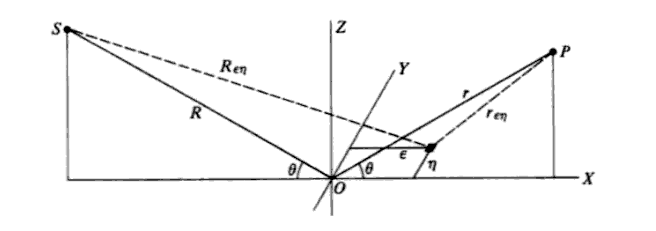
\includegraphics[width=12cm]{pics/picture1.png}
\caption{}
\label{pic1}
\end{center}
\end{figure}

We consider first the reflection from a single layer of unit cells in the Bragg case. Let the incident beam be $\sigma$-polarized (i.e. the electric field is parallel to the layer) and have a wavelength $\lambda$. We can calculate the amplitude of the reflected and transmitted beams by considering the radiation scattered from an element of area $d\epsilon d\eta$ and integrating over the layer. We obtain the following expression for the instantaneous value of the electric field at point $P$ (figure \ref{pic1})

\begin{equation}
 E_P=-ig_\mathbf{H}E_Oe^{(2\pi i /\lambda)[(R+r)-ct]}.
\end{equation}

We introduced the abbreviation

\begin{equation}\label{eqg}
 g_\mathbf{H}=r_e\frac{\lambda F_\mathbf{H}d}{V \sin{\theta_B}}
\end{equation}

where $r_e=\frac{e^2}{mc^2}=2.818 \cdot 10^{-5} \AA{}$ is the classical electron radius, $F_\mathbf{H}$ is the structure factor for the reciprocal lattice vector $\mathbf{H}$, $d$ is the spacing of the reflecting planes, $V$ is the volume of the unit cell and $\theta_B$ is the Bragg angle.

\begin{figure}[h]
\begin{center}
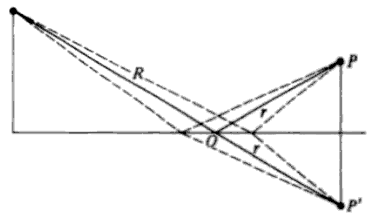
\includegraphics[width=9cm]{pics/picture2.png}
\caption{}
\label{pic2}
\end{center}
\end{figure}


Similarly, the electric field in the beam which has passed through a layer of unit cells is expressed by
\begin{equation}\label{Et}
 E_{P'}=(1-ig_0)E_Oe^{(2\pi i /\lambda)[(R+r)-ct]}
\end{equation}

where
\begin{equation} \label{eqg0}
 g_0=r_e\frac{\lambda F_0 d}{V \sin{\theta_B}}.
\end{equation}

Since $V$ is of order $d^3$, $g_\mathbf{H}$ and $g_0$ are of order $r_0/d \simeq 10^{-5} \ll 1$.

\subsection{Diffraction from a set of atomic planes}
We now turn our attention to the problem of how to calculate the scattering from an infinite stack of atomic planes, where each one reflects and transmits the incident wave according to the equations given in section \ref{onelayer}. The planes are labelled by the index $r$, with the surface plane defined by $r=0$. The objective is to calculate the amplitude reflectivity, which is the ratio of the total reflected wavefield $S_0$ to that of the incident field $T_0$.

Both outside and within the crystal there are two wavefields: the $T$ field propagating in the direction of the incident beam , and the $S$ field in the direction of the reflected beam (figure \ref{pic3}).

\begin{figure}[h]
\begin{center}
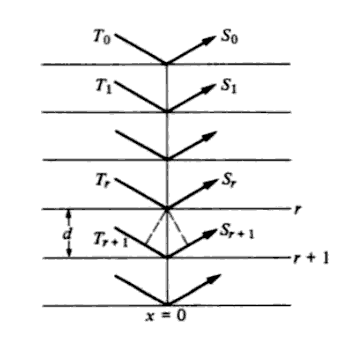
\includegraphics[width=7cm]{pics/picture3.png}
\caption{}
\label{pic3}
\end{center}
\end{figure}


The derivation of Bragg's law relies on the fact that the reflected wave from layer $r+1$ is in phase with the one from layer $r$ if the pathlength differs by an integer number of wavelengths. 
\begin{equation}\label{bragg}
 2\sin{\theta_B}=m\lambda
\end{equation}

As we are interested in deriving the (small) bandwidth of the reflecting region, the phase is restricted to small deviations about $m\pi$, and the phase is given by
\begin{equation}\label{phase}
 \phi=m\pi+\Delta
\end{equation}
where $\Delta$ is a small parameter. In our development of Darwin's theory $\Delta$ will be used as the independent variable.

Let the $T$ field just above layer $r$ on the $z$ axis be denoted $T_r$, and similarly for $S_r$. On being transmitted through the $r$th layer, the $S$ field just above layer $r+1$ changes its phase according to equation \ref{Et}, so that $S_r$ can be written as $(1-ig_0)S_{r+1}e^{i\phi}$. To obtain the total field, we must also add the part due to the reflection of the wave $T_r$. In total then we have
\begin{equation}\label{eq:TS1}
 S_r=-ig_\mathbf{H}T_r+(1-ig_0)S_{r+1}e^{i\phi}
\end{equation}

Next consider the $T$ field just below the $r$th layer. The phase is shifted by $\phi$. This field is composed of contributions from the field $T_r$ after it has been transmitted through the $r$th layer, and from the wave $S_{r+1}e^{i\phi}$ after it has been reflected from the bottom of the $r$th layer. This leads to the second difference equation
\begin{equation}\label{eq:TS2}
 T_{r+1}e^{-i\phi}=(1-ig_0)T_r-ig_\mathbf{\bar{H}}S_{r+1}e^{i\phi}
\end{equation}

A suitable trial solution for \ref{eq:TS1} and \ref{eq:TS2} including a phase shift and attenuation has the form
\begin{equation}
T_{r+1}=e^{-\chi}e^{im\pi}T_r
\end{equation}
\begin{equation}
S_{r+1}=e^{-\chi}e^{im\pi}S_r
\end{equation}
where $\chi$ is a general complex. We can now insert our trial solution into the equations. Noting that $e^{-i\phi}=e^{-im\pi}e^{-i\Delta}$ and expanding all the small parameters to second-order terms yields

\begin{equation}
\chi^2=g_\mathbf{H}g_\mathbf{\bar{H}}-(\Delta-g_0)^2
\end{equation}
which has the solution
\begin{equation}
i\chi=\pm \sqrt{(\Delta-g_0)^2-g_\mathbf{H}g_\mathbf{\bar{H}}}.
\end{equation}

We can now calculate the amplitude reflectivity by inserting our solutions into equation \ref{eq:TS1}. Let $g$ be equal to $\sqrt{g_\mathbf{H}g_\mathbf{\bar{H}}}$. We obtain
\begin{equation}\label{eq:r}
X_R=\frac{S_0}{T_0} \simeq \frac{g}{i\chi+(\Delta-g_0)}
\end{equation}
In order to obtain explicit formulae for the Darwin reflectivity curve the variable $\eta$ is introduced and defined by
\begin{equation}
\eta=\frac{\Delta-g_0}{g}.
\end{equation}
From equation \ref{eq:r} the amplitude reflectivity curve in terms of $\eta$ is
\begin{equation}\label{eq:darwin}
 X_R=\frac{S_0}{T_0}=
 \begin{cases}
  \eta-\sqrt{\eta^2-1} & \quad \text{for } \eta\ge 1  \\
  \eta-i\sqrt{1-\eta^2} & \quad \text{for } |\eta|\le 1  \\
  \eta+\sqrt{\eta^2-1} & \quad \text{for } \eta\le -1  \\
 \end{cases}
\end{equation}


%picture

\subsection{General case: substrate}
%picture
In general the surface of the crystal will not be parallel to the atomic planes which reflect the incident beam, as shown in picture X. This implies a compression of the width of the exit beam. The asymmetry parameter $b$ is defined as
\begin{equation}
 b=\frac{\gamma_0}{\gamma_\mathbf{H}}
\end{equation}
where $\gamma_0$ is the cosine of the angle between the incident beam and the surface normal and $\gamma_H$ is the cosine of the angle between the diffracted beam and the surface normal (in the Bragg case $b$ is always negative).

Equation \ref{eq:darwin} is still valid in the asymmetric case if we include the asymmetric parameter in the variable $\eta$ as follows
\begin{equation}\label{asymm}
 \eta=\frac{-b\Delta-g_0(1-b)/2}{|b|^{1/2}g}
\end{equation}

From equations \ref{bragg} and \ref{phase} and using the fact that $\Delta$ is small we obtain
\begin{equation}\label{Delta}
 \Delta=\frac{2\cos{\theta_B} \pi d}{\lambda}(\theta-\theta_B)
\end{equation}
Substitution of the expressions \ref{eqg}, \ref{eqg0} and \ref{Delta} into equation \ref{asymm} leads to a new expression for $\eta$
\begin{equation}\label{eta}
 \eta=\frac{-b(\theta-\theta_B) \sin{2 \theta_B}-\frac{1}{2}\Gamma F_0(1-b)}{|b|^{1/2}C\Gamma(F_\mathbf{H}F_\mathbf{\bar{H}})}.
\end{equation}


\subsection{General case: epitaxial layer}
In a similar way it is also possible to use dynamical theory to calculate the reflected and transmitted amplitude ratios ($X_R$ and $X_T$) for layers of arbitrary thickness $t$. For convenience we introduce the parameters
\begin{equation}
 T=\pi \Gamma (F_\mathbf{H}F_\mathbf{\bar{H}})^{1/2}\frac{t}{\lambda |\gamma_0 \gamma_\mathbf{H}|^{1/2}}
 \end{equation}
\begin{equation}
 \alpha=T(\eta^2-1)^{1/2}
 \end{equation}
\begin{equation}
 Q=(\eta^2-1)^{1/2}\cos{\alpha} +i\eta \sin{\alpha}.
\end{equation}
where $\eta$ is the variable we defined in equation \ref{eta}.

The equations for $X_R$ and $X_T$ reduce to
\begin{equation}
 X_R=\frac{i \sin{\alpha}}{Q}
 \end{equation}
\begin{equation}
 X_T=\frac{(\eta^2-1)^{1/2}}{Q}.
\end{equation}





\subsection{Recursion formulae}
%picture, more words
When an epitaxial layer with reflected and transmitted amplitude ratios $X_R^1$ and $X_T^1$ is added to a substrate with ratios $X_R^0$, $X_T^0$, the new amplitude ratios $X_t$, $W$ for the crystal can be derived in a recursive way as follows
\begin{equation}
 X_t=X_T^1 Y+X_R^1
\end{equation}
\begin{equation}
 Z=X_R^1 Y+X_T^1
\end{equation}
\begin{equation}
 Y=X_R^0 Z
\end{equation}
\begin{equation}
 W=X_T^0 Z.
\end{equation}

After substitution, we obtain the reflected and transmitted amplitude ratios for the sample
\begin{equation}\label{refl}
 X_t=\frac{X_R^1-X_R^0({X_R^1}^2-{X_T^1}^2)}{1-X_R^0 X_R^1}
\end{equation}
\begin{equation}\label{trans}
 W=\frac{X_T^0 X_T^1}{1-X_R^0 X_R^1}.
\end{equation}






\section{Implementation}

In order to simulate the rocking curves of strained crystals, multilayers and superlattices in the dynamical theory, a Python program has been developed. It is applicable to any coplanar and non-coplanar Bragg-case geometry (see section \ref{geom}) and to crystals with any number of different layers. Layers with arbitrary strain profile are also implemented (see section \ref{strcr}). At the moment perpendicular ($\sigma$) polarization is the only one enabled, but parallel ($\pi$) and mixed polarizations may be included in the future. The program requires \textit{pyasf} () for the definition of the crystal structure and for the calculation of the structure factors.

%something about pyasf

\subsection{Structure}
The program calculates the reflected and transmitted amplitude ratios for an instance object of the class \textit{Sample}. A \textit{Sample} object is nothing but a sequence of other objects of the class \textit{Epitaxial\_Layer}.

For each \textit{Epitaxial\_Layer} the following attributes have to be given:
\begin{itemize}
 \item \textbf{structure} of the crystal, which is taken from a \textit{.cif} file
 \item \textbf{thickness} of the layer in Angstrom
 \item \textbf{R} matrix, i.e. a rotation matrix containing information about the orientation of the unit cell with respect to the surface of the sample
 \item \textbf{Miller} indices of the considered Bragg reflection.
\end{itemize}

A special type of \textit{Epitaxial\_Layer} is defined by the class \textit{Substrate}. The thickness of a \textit{Substrate} is set to be infinity and the trasmitted amplitude is zero. A \textit{Sample} is then made of a \textit{Substrate} object and a list of \textit{Epitaxial\_Layer} objects.

Once the energy and the Miller indices (with respect to the substrate) are given by the user, it is possible to calculate the $\mathbf{q}$ vector in the sample system by using rotation matrices. The Miller indices with respect to a layer are then the integers which best approximate the coordinates of the $\mathbf{q}$ vector in the reciprocal lattice system of the crystal.

%code?

\subsection{Geometrical parameters}\label{geom}

%picture!

Let $\mathbf{a}$, $\mathbf{b}$ and $\mathbf{c}$ be the lattice vector and $\mathbf{a^*}$, $\mathbf{b^*}$ and $\mathbf{c^*}$ the reciprocal lattice vectors.
Let $\hat{x}$, $\hat{y}$ and $\hat{z}$ be the unit vectors of the sample system, such that the normal to the sample surface is parallel to $\hat{z}$ and that $\hat{x}$ lies on the scattering plane.
The geometry of the crystal layers can be specified in 2 different ways.
The user can set the coordinates in the reciprocal lattice system of two vectors $\mathbf{v_\perp}$ and $\mathbf{v_\parallel}$ which are respectively parallel to $\hat{z}$ and $\hat{x}$. The two vectors given should be perpendicular by definition. If this is not the case an error message is printed. To prevent this, the user can give as input an angle $\psi$, which is the angle between $\mathbf{v_\parallel}$ and a reference vector $\mathbf{p}$. The vector $\mathbf{p}$ is defined as the vector perpendicular to $\mathbf{b^*}$ and $\mathbf{v_\perp}$:
\begin{equation}
 \mathbf{p}=\mathbf{b^*} \times \mathbf{v_\perp}.
\end{equation}
If $\mathbf{b^*}$ and $\mathbf{v_\perp}$ are parallel then $\mathbf{p}$ is defined as
\begin{equation}
 \mathbf{p}=\mathbf{v_\perp} \times \mathbf{c^*}
\end{equation}
Specification of $\mathbf{v_\parallel}$ is no longer required since it can be calculated from $\psi$. Now $\mathbf{v_\parallel}$ is automatically perpendicular to $\mathbf{v_\perp}$ and no errors occur.

%details?
%code?
%something about M and R

\subsection{Strained crystals} \label{strcr}
The recursion formulae (\ref{refl}) and (\ref{trans}) can be used for samples made of different epitaxial layers, but also hold for a single crystal with a given strain profile. The strained crystal is treated as a stack of layers with constant strain.


\section{Results}

\subsection{Rocking curves of crystalline multilayers}

\subsection{Diffraction profiles of strained crystals}

\subsection{Comparison with experimental data}



\clearpage 



\nocite{*}
\bibliographystyle{unsrt} 
\addcontentsline{toc}{section}{References}
\bibliography{Elements_of_Modern_X_ray_Physics,X_ray_Diffraction,bartels}{}



\end{document}
